\graphicspath{ {imgs/} }
\documentclass[../Thesis.tex]{subfiles}
\begin{document}
\chapter{Dataset}\label{chap:data}
The Lung Image Database Consortium image collection (LIDC-IDRI) is a publicly available dataset that was generated through the joined effort of seven academic centers and eight medical imaging companies and that contains $1018$ cases. It consists of diagnostic and lung cancer screening thoracic computed tomography (CT) scans with marked-up annotated lesions. More information on the origin of the dataset can be found in the appendix~\ref{appendix:lidc} and the reference paper by Armato~\cite{armato2011lung}. The following sections provide an overview of the data structure and the implemented preprocessing.

\section{Content and Structure}
The dataset contains a folder for each patient. These folders contain a full chest CT scan and the annotations by the radiologists. The CT scan data is encoded in a list of DICOM (Digital Imaging and Communications in Medicine) files and the annotations as one XML (extended markup language) file. The structure of both file types is described in the upcoming sections. More details on how the dataset was formed and how the images are generated by the scanners as well as the parameters that play into that can be found in Appendix~\ref{appendix:data} and \ref{appendix:scanner}.

\subsection{Scan Data Structure}
DICOM is a file format for storing medical images with for the use case relevant meta information. It is not only used for CT scans but also for radiography, ultrasonography and MRI data. It was initially introduced by the American College of Radiology (ACR) and National Electrical Manufacturers Association (NEMA) under the name ACR/NEMA 300 in 1985, but further redefined and finally in the third version released under the name DICOM in 1993\cite{pianykh2008}.

The cases that scans are provided for in the dataset fulfill certain criteria. The CT scans are exclusive of the lung and do not contain other body parts or organs. The reconstruction interval and collimation are kept at $<3$mm. This means that there are differences in the resolution of the scan data (naturally through the different equipment used during recording), but that it is limited with an upper bound. Still one can find patients with $124-529$ recorded images in the data. The scan data may also include noise or other disruptive factors like metal (heart pacers e.g.) as well as other pathological features as long as those do not interfere with the visibility of the nodules in a drastic sense.

The included cases have between $0$ and $6$ nodules with the longest diameter of between $3-30$ mm. The term nodule refers to a brought spectrum of tissue abnormalities and can represent not only lung cancer but also other metastatic diseases or non-cancerous processes or lesions that have a nodular morphology. Typical slices from the data can be seen in Figure~\ref{fig:slices}.

\begin{figure}[!tbp]
\centering
\begin{minipage}[b]{0.7\textwidth}
	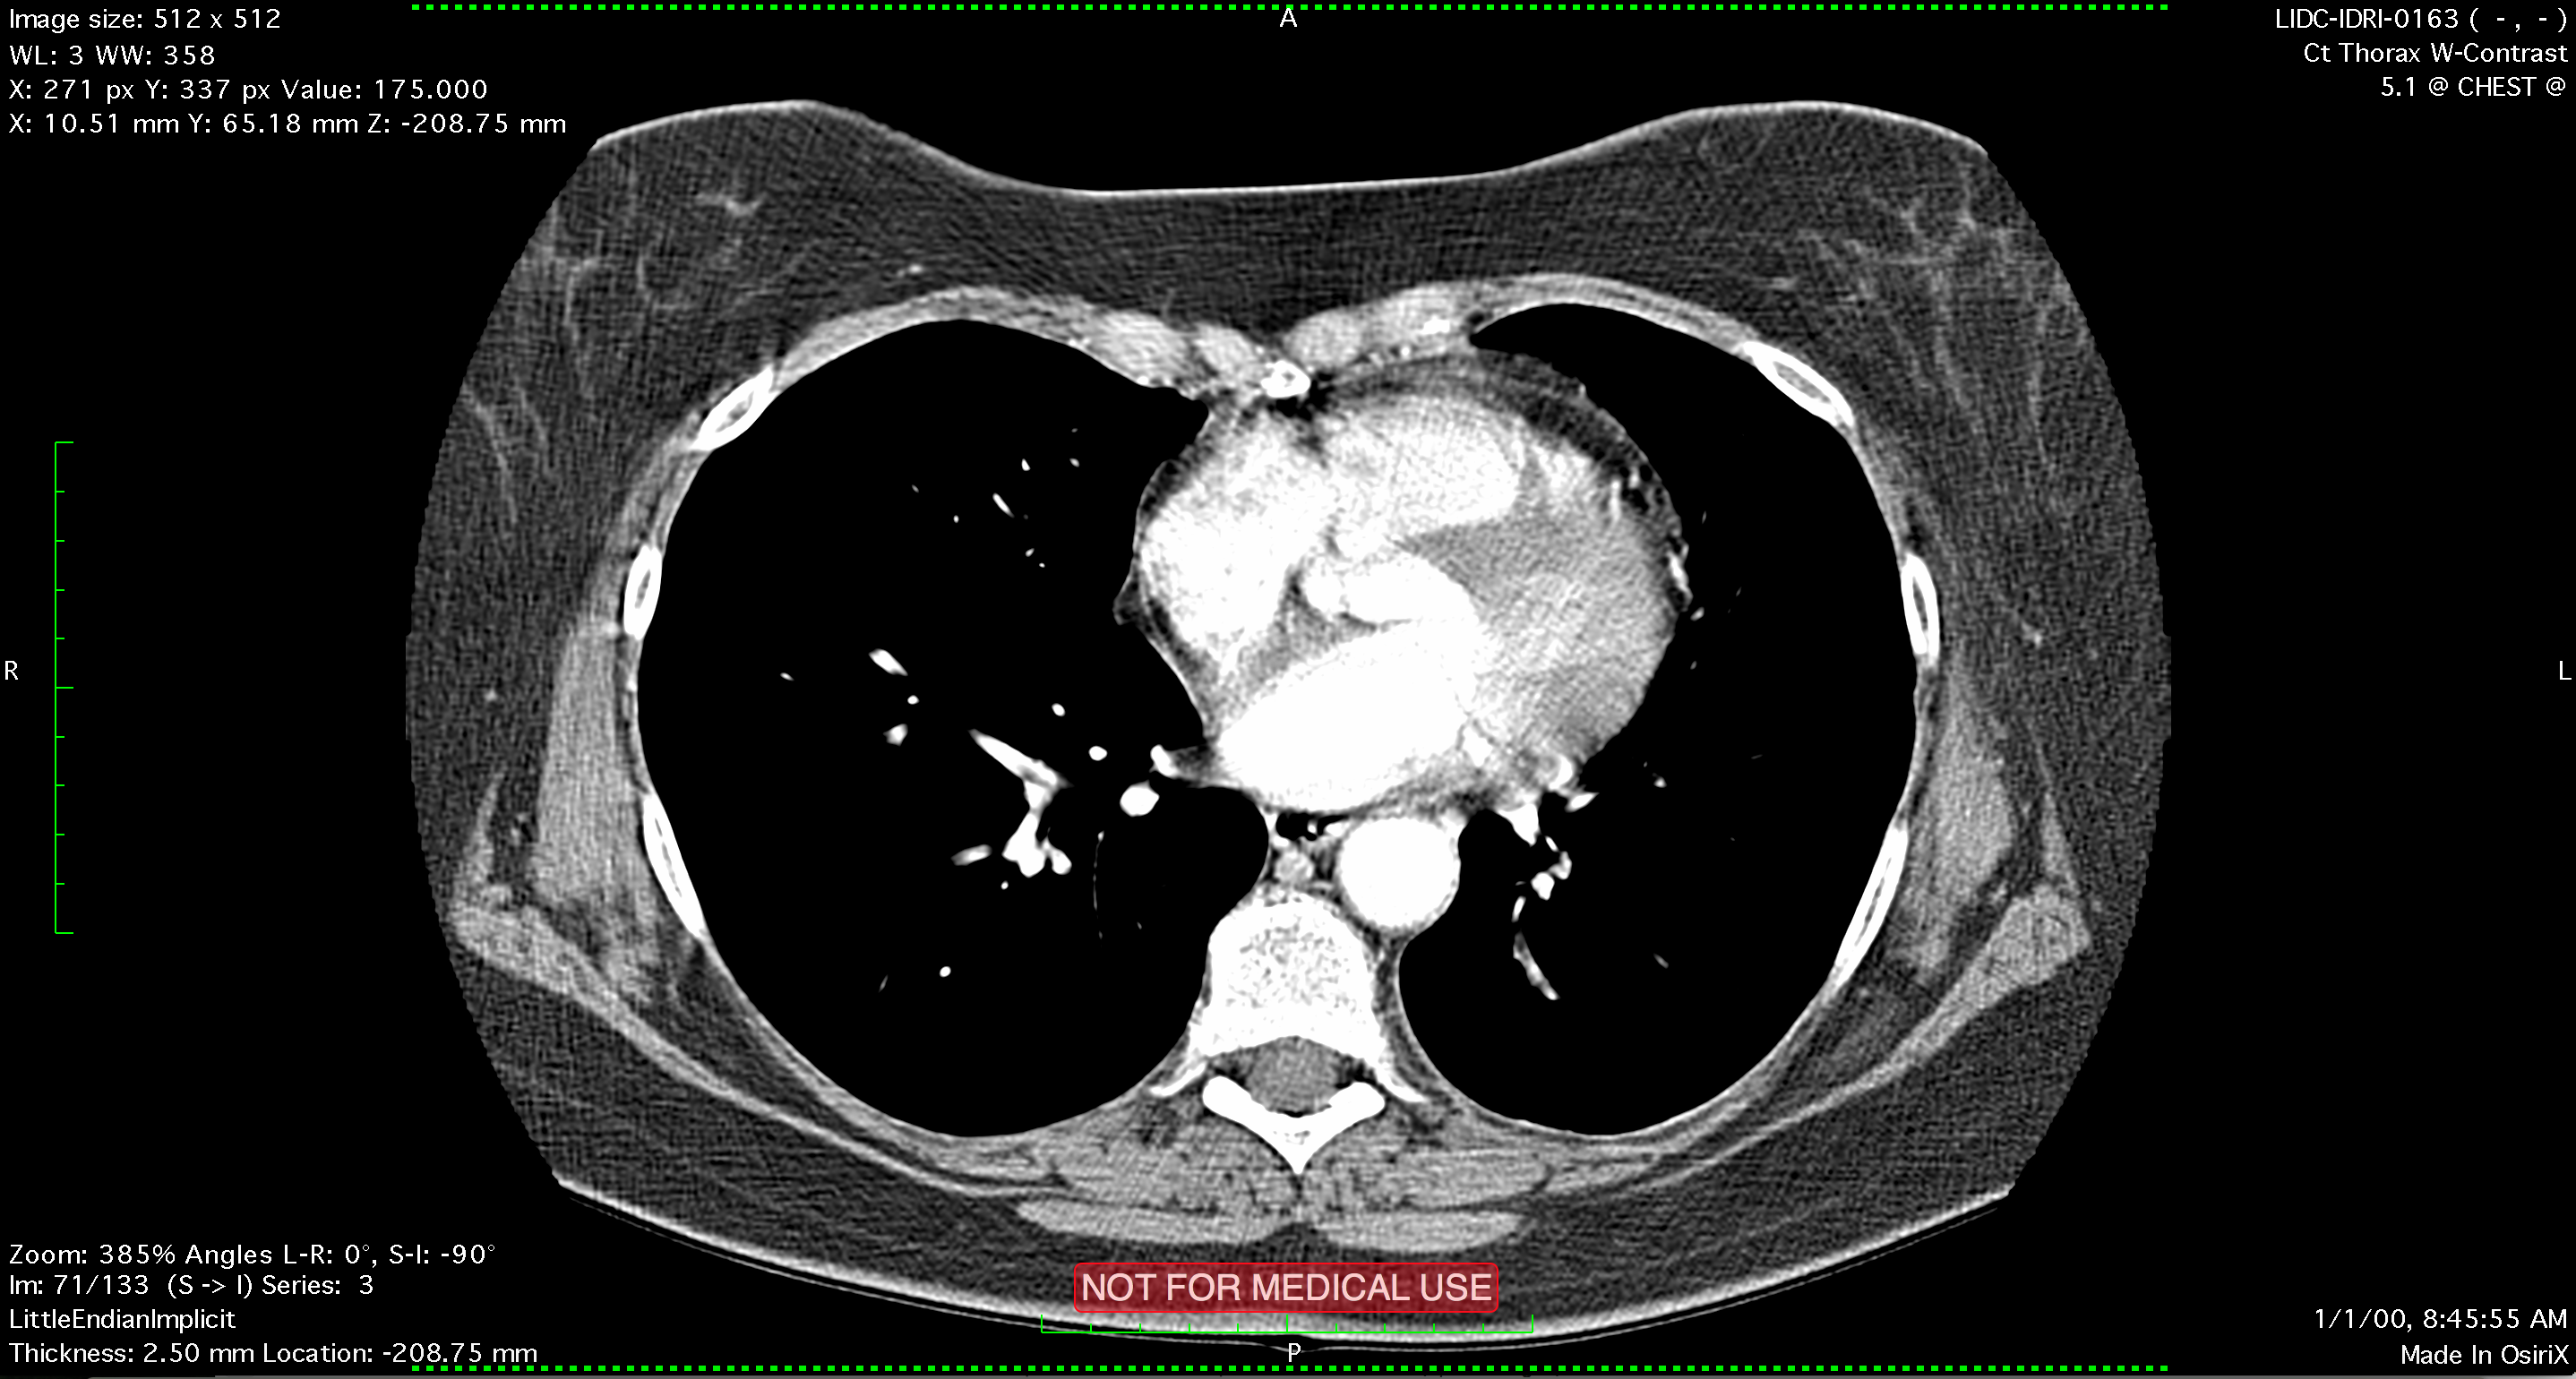
\includegraphics[width=\textwidth]{slice1.png}
\end{minipage}
\begin{minipage}[b]{0.7\textwidth}
	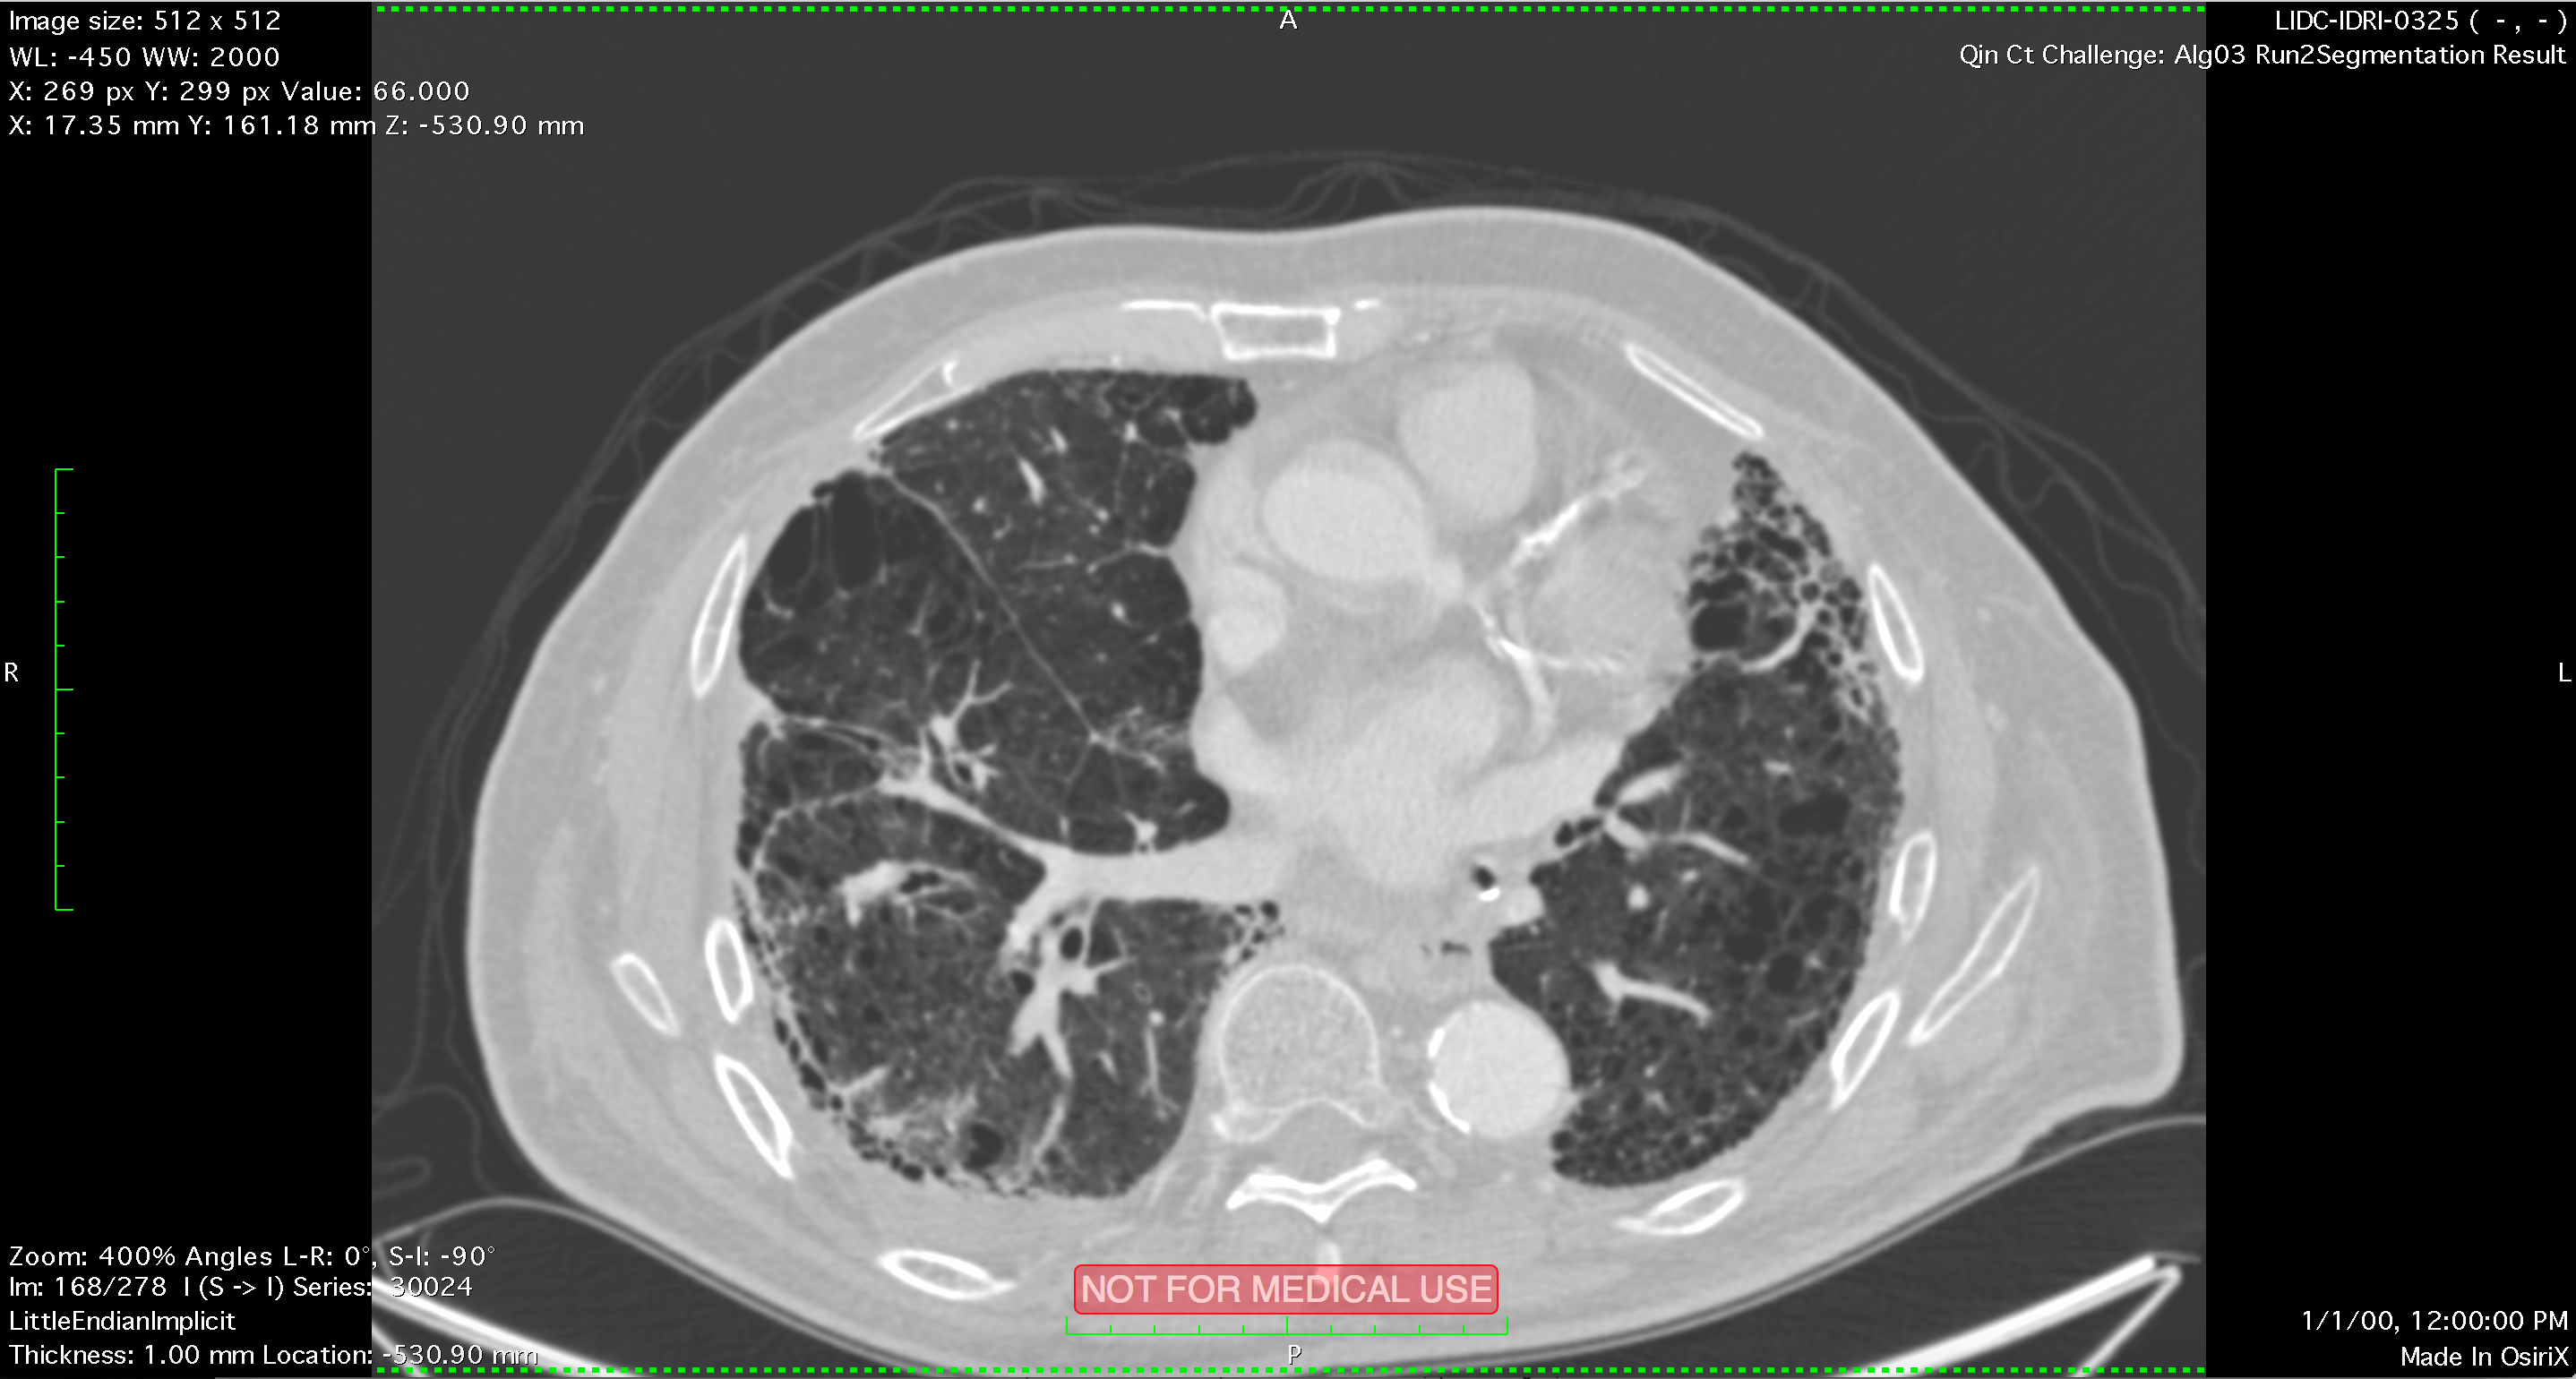
\includegraphics[width=\textwidth]{slice2.png}
\end{minipage}
\caption{Two slices from different patients in the dataset. Images have been generated with OsiriX Lite~\cite{rosset2004osirix}. The information in the corner of the picture is extracted from the meta information stored in the DICOM format.}
\label{fig:slices}
\end{figure}

The additional information about the patients that is usually stored with the scans (like age, name, gender) is anonymized in this dataset.

\subsection{Annotation Structure}
Two different types of nodules are encoded in the data: nodules with a diameter of $>=3$ mm and nodules smaller than that. The big nodules have extensive information stored with them: a rich edge map which outlines a complete contour for them in all sections (as seen in Figure~\ref{fig:bigNod}) and a measure for their characteristics (like their subtlety and malignancy on a scale from 1 to 5). This extra information has not been used in the learning process for this thesis but enables research on further classification and localization tasks.

\lstset{
  language=XML,
  morekeywords={characteristics,noduleID,edgeMap,imageZposition}
}
\begin{figure}
\begin{lstlisting}
      <noduleID>IL057_127581</noduleID>
      <characteristics>
        <subtlety>4</subtlety>
        <malignancy>3</malignancy>
        [...]
      </characteristics>
      
      <edgeMap>
        <xCoord>103</xCoord>
        <yCoord>391</yCoord>
      </edgeMap>
 
      <imageZposition>-232.535004</imageZposition>
       
      <edgeMap>
         <xCoord>104</xCoord>
         <yCoord>393</yCoord>
      </edgeMap>
\end{lstlisting}
\caption{A shortened example XML annotation for a nodule with diameter $>=$ 3mm.}
\label{fig:bigNod}
\end{figure}

Nodules with a smaller diameter have less information stored with them. They only contain the approximate center of mass for the nodule as seen in Figure~\ref{fig:smallNod}.

\begin{figure}
\begin{lstlisting}
	<noduleID>7</noduleID>
	<roi>
	<imageZposition>-227.535004</imageZposition>
        <imageSOP_UID>1.3.6.1.4...</imageSOP_UID>
	<inclusion>TRUE</inclusion>
	<edgeMap>
	   <xCoord>127</xCoord>
	   <yCoord>370</yCoord>
	</edgeMap>
	</roi>
\end{lstlisting}
\caption{Nodules with a diameter of $<3$mm have only the center of mass stored.}
\label{fig:smallNod}
\end{figure}

\section{Preprocessing}
The data is available in the form of sub-folders for each patient that contain the CT scan results in DICOM file format and the annotation data as XML files. The following sections describe the read in and slicing of the data.

\subsection{Reading in the data}
The whole dataset was randomly distributed to 3 folders in a $60:20:20$ split ratio: train, validation and test. The training dataset is used during the learning process of the neural network. The validation dataset is used to measure the performance of the network while it is trained on the training dataset. See Figure~\ref{fig:ttdist} for a distribution of values for the two classes.
 
\begin{figure}
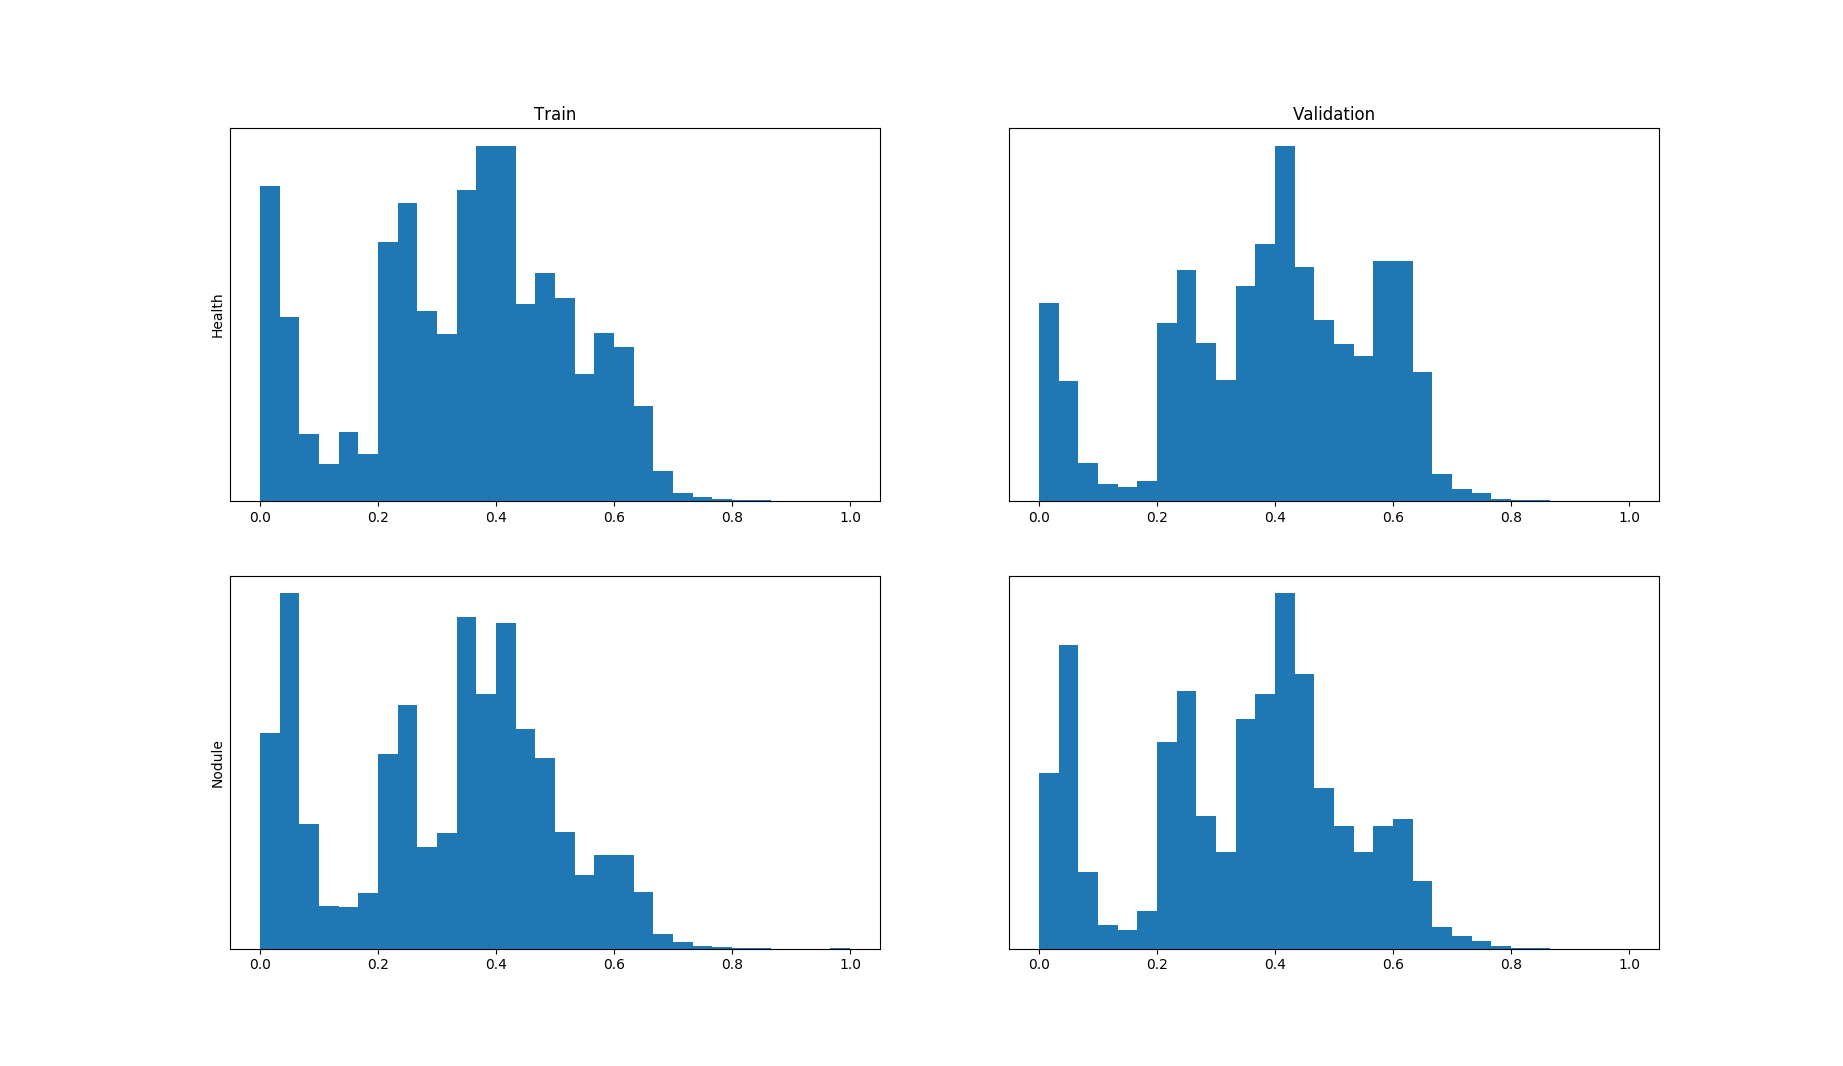
\includegraphics[width=\textwidth]{distribution_class.png}
\caption{Distribution of the normalized pixel values for both classes in the training and validation set (1000 instances per set). This data is used for learning the network.}
\label{fig:ttdist}
\end{figure}

Each of the folders contains a list of patients containing one or more sub-folders with CT scans. Some of the extra folders for a patient contain only a few scans and not a complete CT. Those folders were ignored. With the use of the Python package dicom~\cite{mason2011t} the CT scans are converted to a 3-dimensional array. The annotation XML files are evaluated to find the location of the nodules. In the case of nodules with a diameter of $<3mm$ the center of mass value is used, for the bigger nodules that have information of the whole edge map, the mean over all dimensions is used as an approximation for the center of mass of those nodules. 
$147$ patient files contained no real nodules or had corrupted data (the XML file had a corrupted structure or wrong formatting that prevented the algorithm from extracting the nodule coordinates, one file had a slice thickness of $0$ e.g.). Those files have as well been excluded from the learning process.

\subsection{Slicing the patches}
The information from the annotations is used to generate the patches from the complete scan. A fixed number of patches is generated from the data per patient. The patches for the healthy data are cut randomly from the tissue that contains no nodules while the patches with the nodule information are randomly picked around the nodule's center. Determining the center of a nodule is easy in the cases of the nodules with $<3mm$ diameter. The resulting shape of the patches is $(50,50,5)$. It makes sense to take less value in the z-direction since the resolution of the CT scans is lower in that direction (more information about the scanners can be found in the appendix~\ref{appendix:scanner}).


\end{document}
